\section{Results}
\label{sec:results}
In this section we describe the results obtained from our simulations. 
We have simulated two scenarios: A square room where the pedestrians 
exit through a single door, and pedestrians walking through a corridor 
where there is a bidirectional flow. For each scenario we describe the 
parameters we have set for the scenario, which features we found worth 
measuring for this scenario, the results we expected, and the results 
we obtained. Possible remedies for any discrepancies between the expected 
and the actual results are discussed in section~\ref{sec:discussion}.

\subsection{Constants and scenarios}
We will here shortly specify the values for the different constants 
we use in both of the scenarios and show screenshots of the scenarios 
we will use.

\begin{figure}[h]
\centering
\subfloat[A screenshot of the s]{\begin{tikzpicture}

\end{tikzpicture}
}
\subfloat[]{\begin{tikzpicture}

\end{tikzpicture}
}\\
\subfloat[]{\resizebox{0.45\textwidth}{!}{\begin{tikzpicture}
\draw[color=blue] (10.20,-0.82) circle (0.21);
\draw[color=blue] (11.02,-1.97) circle (0.20);
\draw[color=blue] (9.63,-0.94) circle (0.20);
\draw[color=blue] (11.62,-0.29) circle (0.19);
\draw[color=blue] (11.47,2.10) circle (0.18);
\draw[color=blue] (10.48,-2.41) circle (0.19);
\draw[color=blue] (5.77,0.15) circle (0.20);
\draw[color=blue] (9.33,1.17) circle (0.20);
\draw[color=blue] (11.70,0.48) circle (0.20);
\draw[color=blue] (10.58,-0.16) circle (0.20);
\draw[color=blue] (10.44,1.08) circle (0.19);
\draw[color=blue] (12.15,1.00) circle (0.18);
\draw[color=blue] (11.04,1.59) circle (0.19);
\draw[color=blue] (9.23,-0.44) circle (0.19);
\draw[color=blue] (6.84,-1.70) circle (0.20);
\draw[color=blue] (8.87,1.83) circle (0.20);
\draw[color=blue] (6.54,-0.44) circle (0.18);
\draw[color=blue] (10.86,-1.36) circle (0.21);
\draw[color=blue] (9.88,0.21) circle (0.20);
\draw[color=blue] (9.89,-1.87) circle (0.20);
\draw[color=blue] (6.04,-1.63) circle (0.21);
\draw[color=blue] (8.87,0.53) circle (0.21);
\draw[color=blue] (7.99,0.26) circle (0.20);
\draw[color=blue] (5.41,-0.25) circle (0.20);
\draw[color=blue] (11.07,0.44) circle (0.20);
\draw[color=blue] (8.60,-0.27) circle (0.20);
\draw[color=blue] (7.87,1.96) circle (0.19);
\draw[color=blue] (7.11,0.68) circle (0.20);
\draw[color=blue] (8.43,1.00) circle (0.20);
\draw[color=blue] (7.83,-0.50) circle (0.19);
\draw[color=blue] (8.64,-1.20) circle (0.21);
\draw[color=blue] (9.34,-1.40) circle (0.20);
\draw[color=blue] (4.83,-0.64) circle (0.21);
\draw[color=blue] (6.07,-0.86) circle (0.19);
\draw[color=blue] (6.45,0.89) circle (0.21);
\draw[color=blue] (7.89,1.19) circle (0.19);
\draw[color=blue] (1.67,-0.57) circle (0.20);
\draw[color=blue] (6.05,1.61) circle (0.20);
\draw[color=blue] (5.49,-1.13) circle (0.20);
\draw[color=blue] (4.13,0.72) circle (0.20);
\draw[color=blue] (3.48,-0.13) circle (0.20);
\draw[color=blue] (3.54,0.51) circle (0.19);
\draw[color=blue] (4.60,-1.25) circle (0.20);
\draw[color=blue] (3.76,-1.28) circle (0.20);
\draw[color=blue] (5.80,0.82) circle (0.20);
\draw[color=blue] (5.09,0.53) circle (0.18);
\draw[color=blue] (0.27,-0.23) circle (0.19);
\draw[color=blue] (2.15,-0.14) circle (0.18);
\draw[color=blue] (4.12,-0.39) circle (0.20);
\draw[color=blue] (5.03,1.23) circle (0.19);
\draw[color=blue] (2.85,0.76) circle (0.21);
\draw[color=blue] (3.49,1.13) circle (0.19);
\draw[color=blue] (3.39,-0.85) circle (0.21);
\draw[color=blue] (-2.42,-1.28) circle (0.19);
\draw[color=blue] (0.41,0.15) circle (0.22);
\draw[color=blue] (4.91,0.01) circle (0.20);
\draw[color=blue] (2.96,0.05) circle (0.20);
\draw[color=blue] (-1.40,0.87) circle (0.18);
\draw[color=blue] (1.40,-0.17) circle (0.19);
\draw[color=blue] (-0.07,0.31) circle (0.20);
\draw[color=blue] (2.70,-0.66) circle (0.20);
\draw[color=blue] (-0.88,-0.27) circle (0.19);
\draw[color=blue] (1.68,0.44) circle (0.19);
\draw[color=blue] (2.34,0.58) circle (0.20);
\draw[color=blue] (-0.24,-0.22) circle (0.21);
\draw[color=blue] (-0.46,0.41) circle (0.21);
\draw[color=blue] (0.94,-0.05) circle (0.19);
\draw[color=blue] (-0.92,0.14) circle (0.19);
\draw[color=blue] (-0.67,-0.63) circle (0.21);
\draw[color=blue] (-1.38,-0.47) circle (0.19);
\draw[color=blue] (-1.89,0.99) circle (0.21);
\draw[color=blue] (-1.76,0.15) circle (0.20);
\draw[color=blue] (-2.41,1.34) circle (0.20);
\draw[color=blue] (-2.18,-0.65) circle (0.18);
\draw[color=blue] (-0.95,0.61) circle (0.19);
\draw[color=blue] (-1.46,-0.97) circle (0.21);
\draw[color=blue] (-2.67,-0.12) circle (0.19);
\draw[color=blue] (-3.08,-1.51) circle (0.19);
\draw[color=blue] (-4.20,1.96) circle (0.22);
\draw[color=blue] (-3.33,1.39) circle (0.21);
\draw[color=blue] (-3.10,-0.80) circle (0.20);
\draw[color=blue] (-4.15,1.04) circle (0.19);
\draw[color=blue] (-3.71,-1.07) circle (0.22);
\draw[color=blue] (-2.49,0.61) circle (0.19);
\draw[color=blue] (-3.55,-1.91) circle (0.20);
\draw[color=blue] (-3.31,-0.17) circle (0.18);
\draw[color=blue] (-4.55,-0.92) circle (0.21);
\draw[color=blue] (-3.10,0.61) circle (0.20);
\draw[color=blue] (-3.90,0.00) circle (0.20);
\draw[color=blue] (-4.83,1.46) circle (0.21);
\draw[color=blue] (-5.43,0.90) circle (0.20);
\draw[color=blue] (-4.93,-1.33) circle (0.20);
\draw[color=blue] (-4.79,0.18) circle (0.21);
\draw[color=blue] (-5.65,-0.68) circle (0.21);
\draw[color=blue] (-5.97,1.31) circle (0.20);
\draw[color=blue] (-5.56,0.01) circle (0.22);
\draw[color=blue] (-5.76,-1.47) circle (0.20);
\draw[color=blue] (-6.06,0.46) circle (0.19);
\draw[color=blue] (-7.12,1.03) circle (0.20);
\draw[color=blue] (-6.41,-0.92) circle (0.20);
\draw[color=blue] (-7.05,-1.14) circle (0.18);
\draw[color=blue] (-6.56,-0.19) circle (0.21);
\draw[color=blue] (-7.82,-1.02) circle (0.21);
\draw[color=blue] (-7.69,0.99) circle (0.20);
\draw[color=blue] (-7.09,0.32) circle (0.21);
\draw[color=blue] (-7.55,-0.00) circle (0.19);
\draw[color=blue] (-8.21,0.32) circle (0.19);
\draw[color=blue] (-7.85,-0.40) circle (0.19);
\draw[color=blue] (-8.77,0.80) circle (0.19);
\draw[color=blue] (-8.95,-0.09) circle (0.20);
\draw[color=blue] (-9.22,-0.80) circle (0.20);
\draw[color=blue] (-8.59,-0.84) circle (0.21);
\draw[color=blue] (-9.39,0.70) circle (0.20);
\draw[color=blue] (-9.73,0.68) circle (0.21);
%\node at (-12.50, 5.83) {t = 40.26};
\useasboundingbox (-12.50, -5.83) rectangle (12.50, 5.83);
\draw[color=black] (-10.00,3.00) -- (-5.00,3.00);
\draw[color=black] (-10.00,-3.00) -- (-5.00,-3.00);
\draw[color=black] (-5.00,3.00) -- (0.00,0.50);
\draw[color=black] (-5.00,-3.00) -- (0.00,-0.50);
\draw[color=black] (0.00,0.50) -- (5.00,3.00);
\draw[color=black] (0.00,-0.50) -- (5.00,-3.00);
\draw[color=black] (5.00,3.00) -- (10.00,3.00);
\draw[color=black] (5.00,-3.00) -- (10.00,-3.00);
\end{tikzpicture}
}}
\subfloat[]{\begin{tikzpicture}

\end{tikzpicture}
}
\caption{We simulate four different scenarios.}
\label{fig:fourcases}
\end{figure}

In the simulation the parameters are set after \cite{ABconstant} and 
\cite{self-org}, to see if we can replecate their simulations and results. 
The general values we use are

\begin{center}
\begin{table}[ht]
\begin{center}
    \begin{tabular}{ | l | l | l |}
    \hline
       Describtion & Constants & Value \\ \hline \hline
	Strenght of pedestrian repulsion & A & $3.0m/s$ \\ \hline	
	Range of pestrian repulsion & B & $0.2$ \\ \hline
	Anisotropic constant & $\lambda$ & $0.1$ \\ \hline
	Wall constant & $U$ &  $2.0m^2/s^2$ \\ \hline
	Mean desired velocity &  $\langle V^d \rangle$ &  $1.34 m/s$, deviation $0.26 m/s$ \\ \hline
	Max velocity factor & - &  $1.3$ \\ \hline
	Mean radius of pedestrians & R & $0.3 m$, deviation $0.05 m$\\ \hline
	Relaxation time & $\tau$ & $1.0 s$\\ \hline
    \end{tabular}
\label{Table_constants}
\end{center}
\end{table}
\end{center}

We will through the chapter mention when the values are changed for a specific case.  

\subsection{Startup}
Running the first simulations where all about to see if there where any 
unatural behavior by the pedestrians, when using the parameters in table 
\ref{Table_constants}. We checked for intersections between the pedestrians, 
pedestrians crossing the walls and so on.

\begin{figure}[h]
\centering
\subfloat[Pedestrians overlapping]{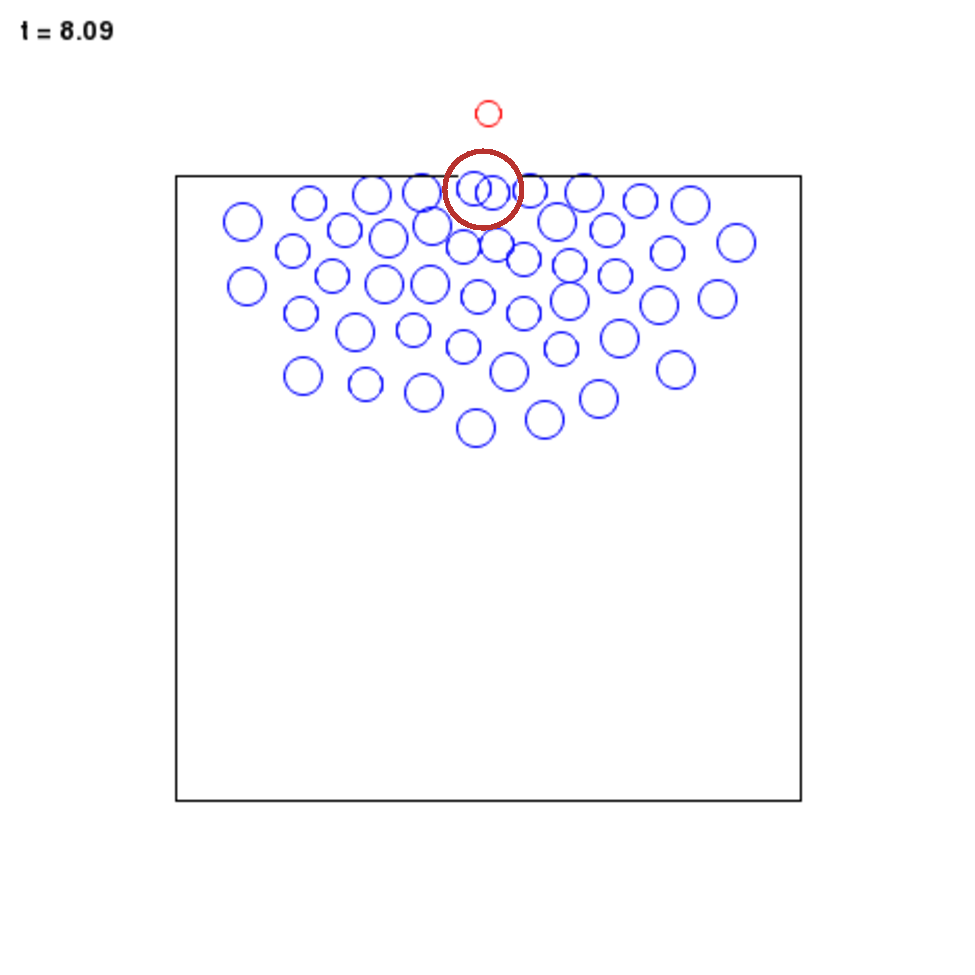
\includegraphics[scale=0.45]{Figures/pedestiranoverlapping.pdf}}
\subfloat[Overlapping between pedestrians and a wall]{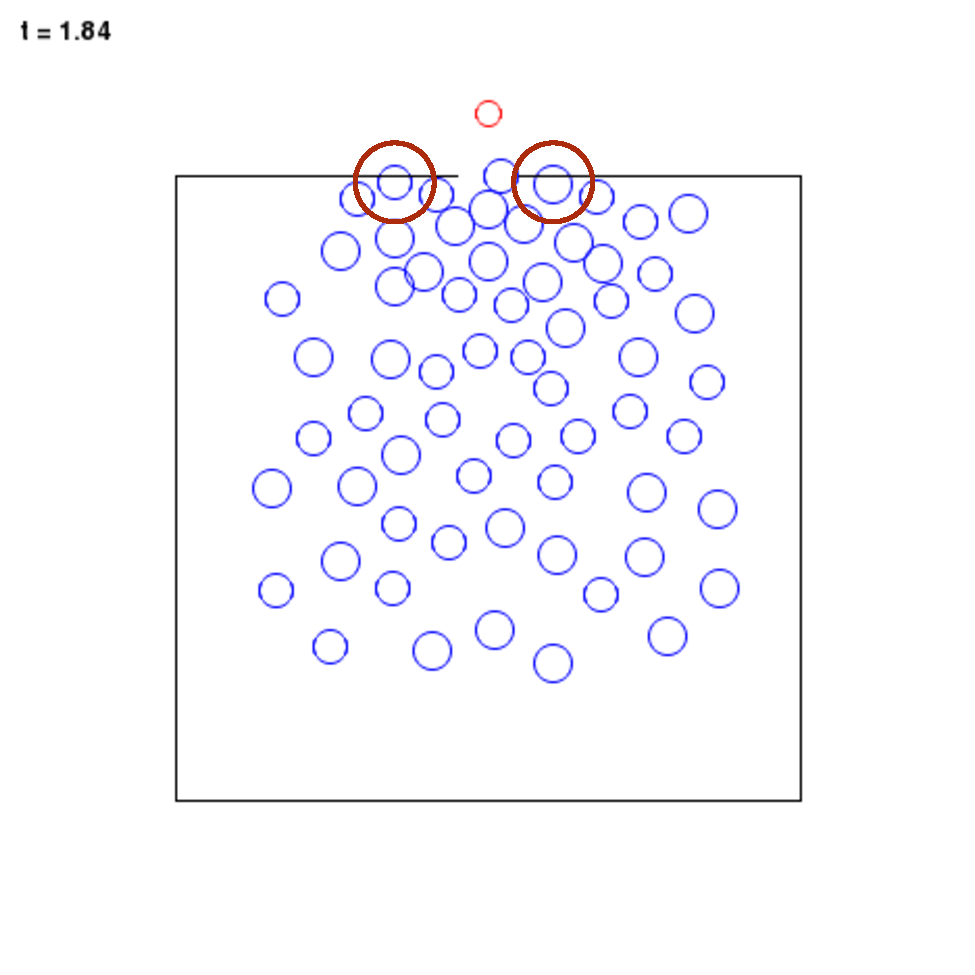
\includegraphics[scale=0.45]{Figures/walloverlapping.pdf}}
\caption{The figure shows two simulations of the squared room. We see the overlapping that can occur between two pedestrians and between the walls and pedestrians. This kind of intersection is seen in most simulations, but they don't cross completely. The red dot on the figures are the desired locations}
\label{fig:overlapping}
\end{figure}

In the figure \ref{fig:overlapping} the overlapping between pedestrians 
themselves and between walls and pedestrians. We see that in some situations 
it is possible for the pedestrians to intersect quite alot, almost reaching 
each others centers. The same thing is seen for the walls, where the wall 
can get quite close to the center of a pedestrians. But inspite of this 
we don't, with the chosen constants, see that they actually do cross. So 
even though it might look like they get sqiuzzed alot together, no completely 
unrealistic situations occur. Also we see no other strange scenarios, like 
people going in a wrong direction or anything like that. So the most basic 
requirements of the model are fulfilled. 

We do however see some unrealistic behavior when we change the values in 
\ref{Table_constants} When looking at some of the different phenomenons, 
we need to change certain values like the mean velocity. But when we do 
this it starts to get unrealistic. When raising the desired velocity to 
a speed like $2.5m/s$, we start to see people crossing each other and going 
up to $3.5m/s$ we start to see people crossing the walls. This is a problem 
since these results makes no sence to compares with. Lowering the timestep 
with $1/10$ doesn't change this result at all. So to solve this problem we 
have in some cases raised the wallues of the wall constant $U$ and the 
pedestrains repulsion constant $A$. This makes the repulsions forces 
big enough for the pedestrians to act 'noraml'. We will throughout the 
chapter mention when we change the values and how much it is changed.



\subsection{The square room scenario}
In this scenario we simulate pedestrians leaving a square room of 10 m by 
10 m with a single $80cm$ wide door. 100 pedestrians are positioned randomly 
throughout the room. The second the simulation start all pedestrians head 
for the exit. The parameters for this simulation are as in \ref{Table_constants}

First the claim of the "faster-is-slower" effect is tested.
\begin{quote}
Even counterintuitive
effects are well reproduced. This includes the “faster is-
slower effect” and stripe formation in intersecting flows. \cite{self-org}
\end{quote}
We would then expect that a high nervousness would lead to slower evacuation, because of additional clogging at the doorway. But this phenomena do not occur in our simulation see figure \ref{FastIsSlow}
\begin{figure}
\centering
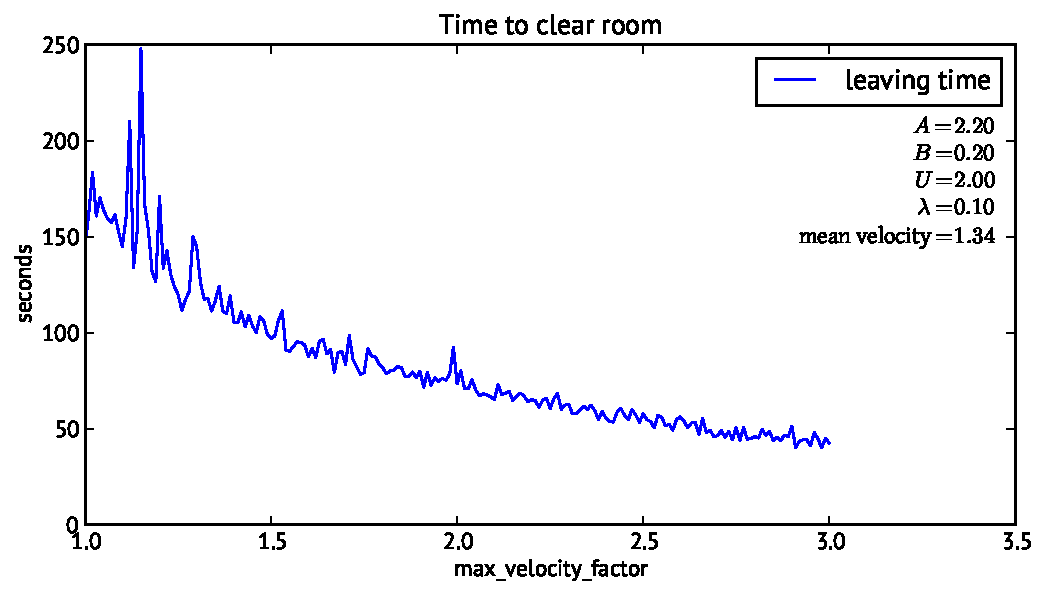
\includegraphics[scale=0.5]{Figures/fastIsSlowNot}
\caption{Fast is not slow}
\label{FastIsSlow}
\end{figure}

The larger the nervousness the faster is the evacuation. We have increased 
the max-velocity factor sow much that people eventually move through the walls. 
This start occurring around max-velocity-factor = 2.5, and measurements beyond 
this point are neglected.

Pedestrian flow rate is measure in the door opening, and the density of pedestrians 
in a 2 m by 2 m area directly in front of the door is measured. We also measure 
the time it takes for all pedestrians to leave the room.

The parameters for this simulation are the ones shown in \ref{Table_constants}

% TODO: Add parameters that are varied.


\subsection{The corridor scenario}
In this scenario we simulate pedestrians walking in both directions along a 20 
m long and six metres wide corridor. The pedestrians are divided into two 
groups, starting in opposite ends of the corridor and moving towards each 
other. The targets the pedestrians move towards are set 500 metres to each 
side, to make pedestrians walk in almost a straight line instead of converging 
towards the middle of the corridor. Flow rate is measured in the middle of the 
corridor, as is density. We start out with 100 pedestrians, adding a 
continuous inflow of three pedestrians per second, to simulate people arriving 
from outside the simulated area. Both the initial placement and the inflow of 
pedestrians are distributed randomly (i.e. approximately evenly) between the 
two ends of the corridor.

We expect to see lane formations through out our simulations
and the freezing by heating effect when we start raising the mean velocity
of the agents.

\subsubsection{Intial conditions and relaxation time $1,0$ second}

The parameters for this simulation are as in \ref{Table_constants} with the exception of the pedestrians
\begin{itemize*}
    \item Number of pedestrians: $40$ starting, adding $3/s$.
\end{itemize*}

When running the simulation we observe lane formations, and they almost clog up
in the corridor.

When we do a simulation with the max velocity factor set to $4.0$, instead 
of the normal $1.3$, the clogging that occurs in the beginning eases up, 
and the pedestrians relatively fast get out of the clogging and continuous 
toward their target. In this simulation we also observe lane formations.

\begin{figure}[h]
\centering
\subfloat[The figure show the density in corridor when the parameters are set as \cite{ABconstant} and \cite{self-org}.]{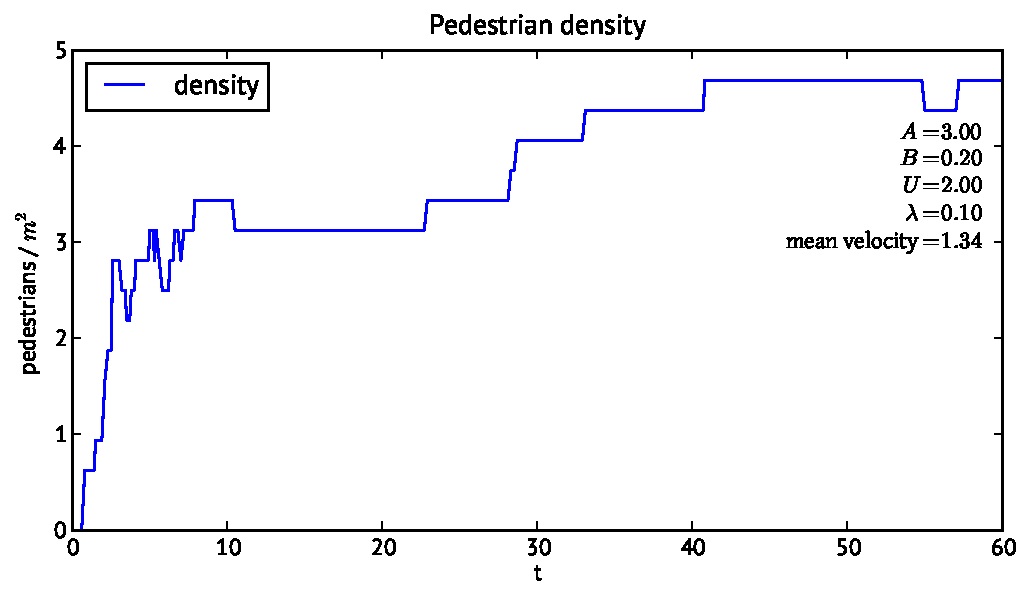
\includegraphics[scale=0.45]{Figures/dens_init_relax1.pdf}}
\subfloat[This figure shows the density in the corridor when the max velocity factor is set to $4.0$, and the other parameters as figure a.]{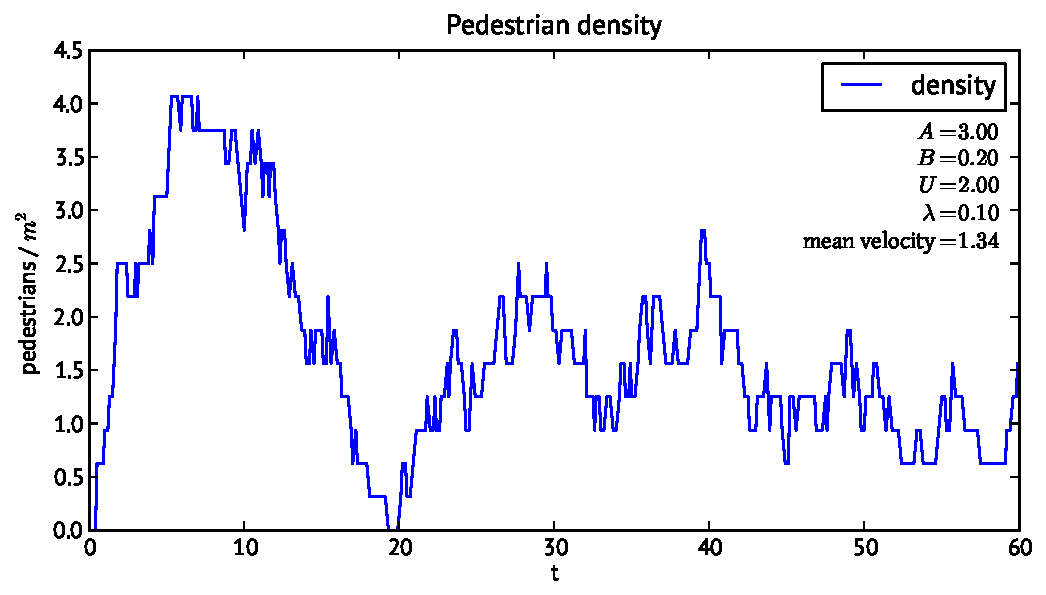
\includegraphics[scale=0.45]{Figures/dens_mvel4_relax1.pdf}}
\caption{These figures was made to see if the freezing by heating effect when raising the max velocity factor. As seen in the figures, the
density does not increase when the max desired velocity is increased. When raising the max desired velocity the density gets lower because
the pedestrians more easely get through the crowd.}
\label{fig:freezingbyheating1}
\end{figure}

\subsubsection{Intial conditions and relaxation time $0,5$ second}
\cite{helbing00} set the relaxation time to $0,5$. As the first corridor simulations we set the parameters as \cite{ABconstant}
and then change the relaxation time to $0,5$ as \cite{helbing00}. After the simulation with the initial conditions, we raise the
max desired velocity to see if we can replicate the freezing by heating effect.

The initial simulation has the values from \ref{Table_constants} with the exceptions:

\begin{itemize*}
    \item Relaxation time: $0,5 s$.
    \item Number of pedestrians: $40$ starting, adding $3/s$.
\end{itemize*}

The next simulation we keep the new relaxation time, but changes the max velocity factor set to $4.0$


When comparing the simulations we do not see the freezing by heating effect.
Instead we see that the pedestrians more easely escape the clogging, and the 
flow in each directionsgets more steady. In both simulations we observed lane 
formation.

\begin{figure}[h]
\centering
\subfloat[The figure show the density in corridor when the parameters are set as \cite{ABconstant} and \cite{helbing00}.]{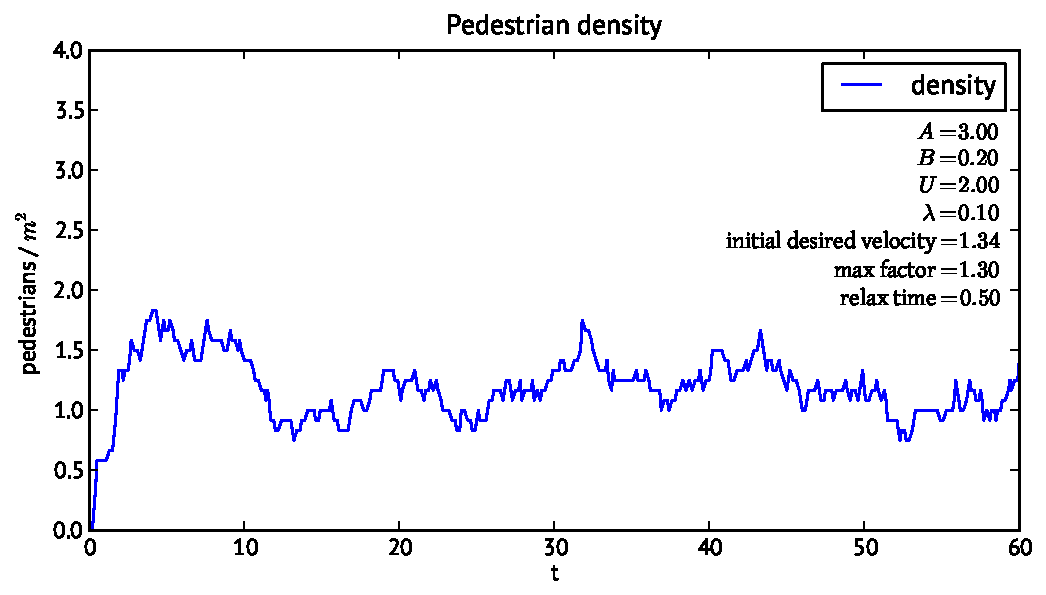
\includegraphics[scale=0.45]{Figures/dens_init_relax05.pdf}}
\subfloat[This figure shows the density in the corridor when the max velocity factor is set to $4.0$ and the max desired velocity is set to $4,0$, and the other parameters as figure a.]{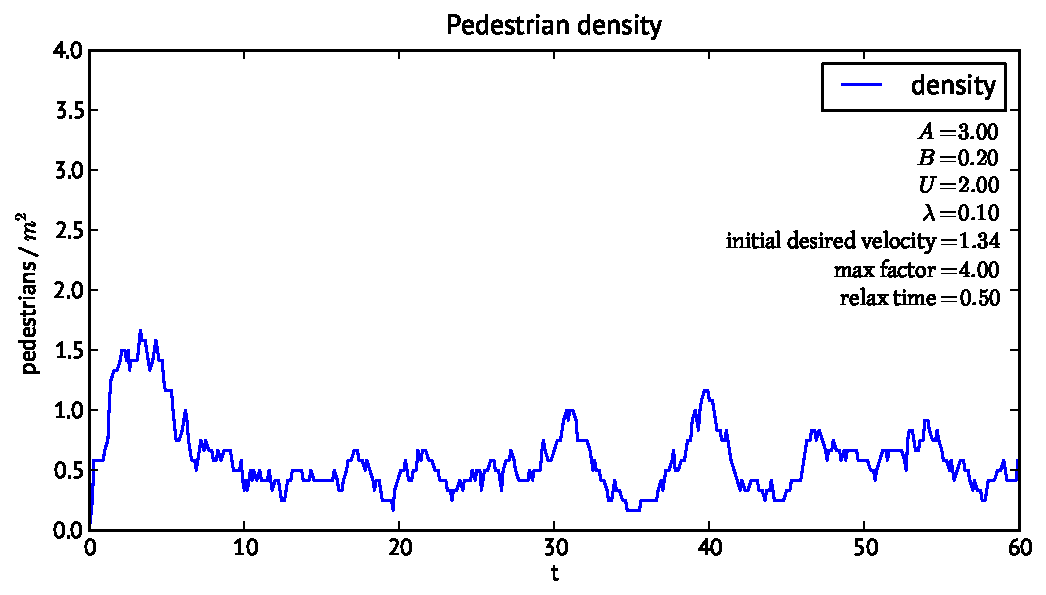
\includegraphics[scale=0.45]{Figures/dens_mvel4_relax05.pdf}}
\caption{These figures was made to see if the freezing by heating effect when raising the max velocity factor. As seen in the figures, the
density does not increase when the max desired velocity is increased. When raising the max desired velocity the density gets lower because
the pedestrians more easely get through the crowd. The difference between figure \ref{fig:freezingbyheating1} and this is the relation time,
respectively $1,0$ and $0,5$.}
\label{fig:freezingbyheating05}
\end{figure}

\subsubsection{Comparison between the relaxation time $1,0$ second and $0,5$ second}
When simulating the corridor with the initial conditions and changing 
the relaxation time from $1,0 s$ to $0,5 s$, the pedestrians do not get 
stuck as easely when the relaxtion time is $0,5 s$ as they do when the 
relaxation time is $1,0 s$. This can be seen in figure 
\ref{fig:comparison_of_timestep}, that in (a), the density get high faster, 
while in (b) the density does not increase as fast as (a). When the 
relaxation time is $0,5 s$, the pedestrians reacts faster, in the sense 
that they speed up faster, after collisions with pedestrians walking in 
the other direction.

\begin{figure}[h]
\centering
\subfloat[The figure show the density in corridor when the relaxation time is set to $1,0 s$]{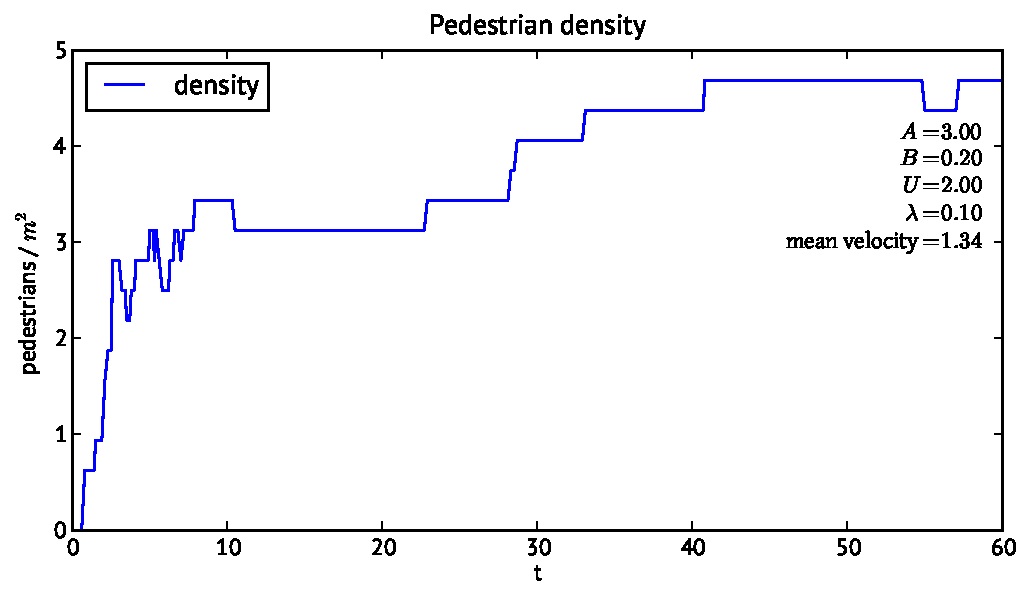
\includegraphics[scale=0.45]{Figures/dens_init_relax1.pdf}}
\subfloat[This figure shows the density in the corridor when the relaxation time is set to $0,5 s$]{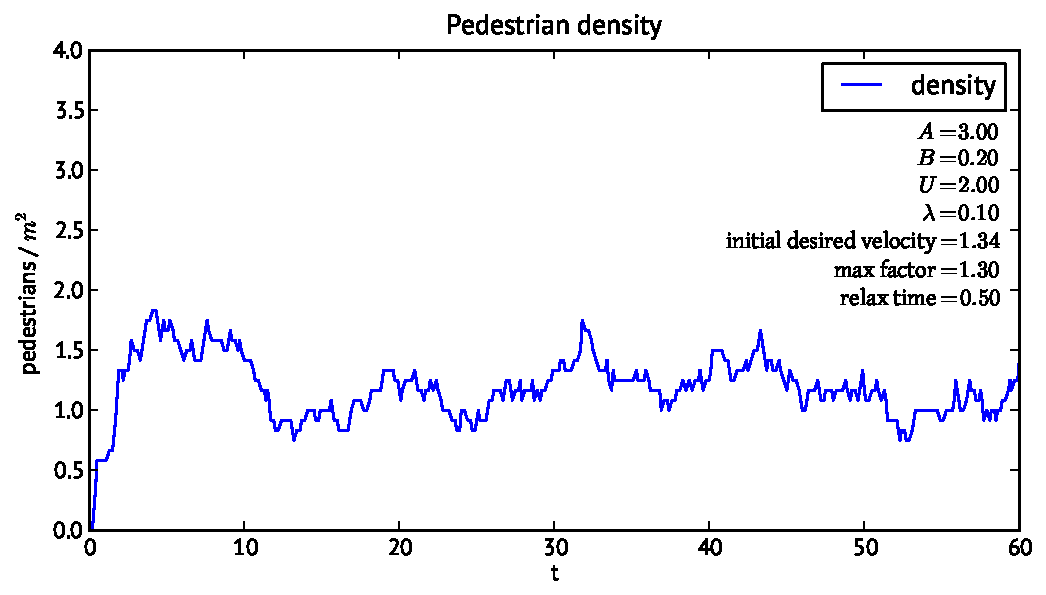
\includegraphics[scale=0.45]{Figures/dens_init_relax05.pdf}}
\caption{These figures show the difference of the density when changing the relaxation time of the model from $1,0 s$ to $0,5 s$.
It is seen the the density is more steady when the relaxtion time is $0,5 s$ instead of $1,0 s$}
\label{fig:comparison_of_timestep}
\end{figure}

A possible explanation of why the density is more steady through out 
the simulation when the relaxation time is $0,5 s$, is that the 
pedestrians reacts faster to changes of their velocity. Thus when they 
bump into each other, they speed up faster, and therefore avoid 
clogging up before more get in their path.

\subsubsection{Freezing by heating effect}
According to \cite{self-org} the freezing by heating effect should 
arise when the max desired velocity of the pedestrians was raised.
That is that clogging should arise when raising the max velocity of 
the pedestrians, because more are ariving to the possible clogging area, 
and thus have more trouble getting through the crowd. We tried to raise 
the max velocity, see figure \ref{fig:freezingbyheating1} and figure 
\ref{fig:freezingbyheating05}, but instead of observing the freezing 
by heating effect, we saw that the pedestrians got through the corridor 
more easely, and that the density in the corridor was lower when the 
max velocity was high. We think that there are more explations to this 
result. For the first the pedestrian $\alpha$'s force toward the target
is higher when $\alpha$'s velocity gets higher, and therefore he more 
easely pushes his way through the crowd. For the second there are no 
friction between the pedestrians to slow $\alpha$ speed down, besides 
the social sphere.

\subsection{The bottleneck}
In this scenario we wanted to the the oscillitory flows that is reported 
in \cite{self-org} to happen when you have a bidirectional flaw through a 
bottleneck.

\subsubsection{The Oscillitory flow}

\begin{figure}[h]
\centering
{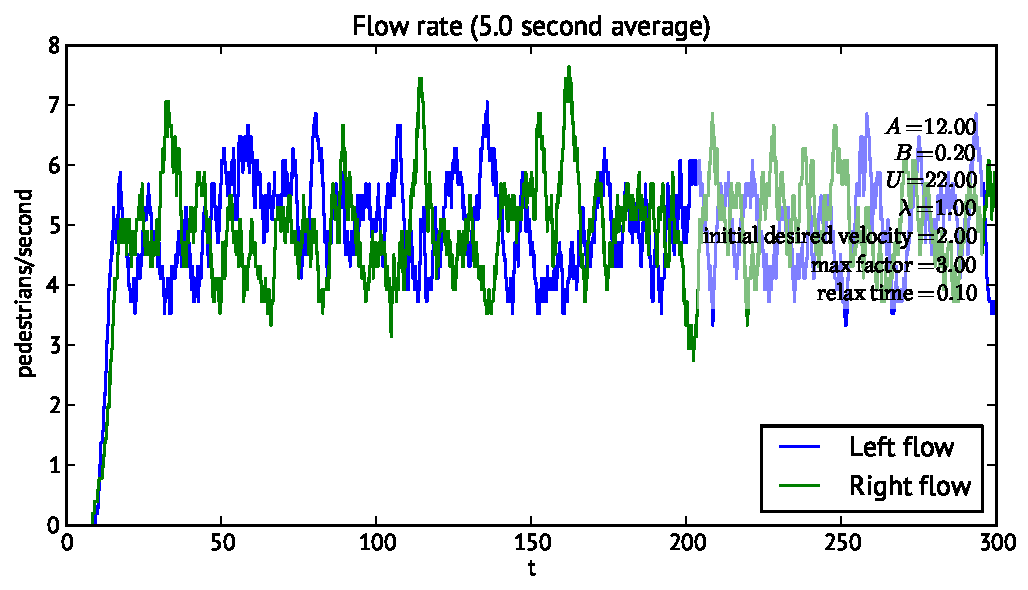
\includegraphics[scale=0.5]{Figures/bottleneck-flowrate-2.pdf}}
\caption{A screen shot of the bottleneck simulation.}
\label{fig:oscillitoryflow}
\end{figure}

\subsubsection{The faster is slower effect in the bottleneck}
In order to see the faster-is-slower effect we make a series of simulations 
with increasing mean velocity. The results is presented in figure 
\ref{fig:is-faster-slower-in-bottleneck}.

\begin{figure}[h]
\centering
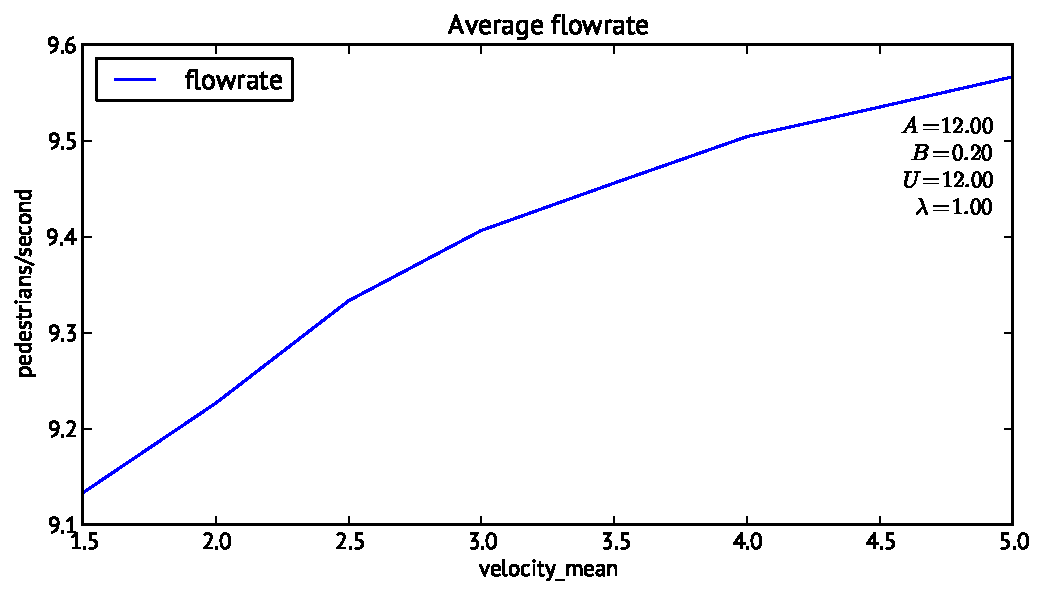
\includegraphics[scale=0.45]{Figures/Wide-kink-one-directional-flowrate-agg.pdf}
\caption{A graph of the flow rate as the average velocity is increased}
\label{fig:is-faster-slower-in-bottleneck}
\end{figure}

\subsection{The corridor with open space}
In this scenario we wanted to reproduce the results that people start to 
clock up in a corridor if there is a sudden area that allow pedestrians to try 
and overtake each other. To see if the flow rate is affected by the pedestrians 
who try to overtake each other we compare the flow rate with the wide space with 
the flow rate from a normal corridor scenario.

\begin{figure}[h]
\centering
\subfloat[A graph of the mean velocity of the pedestrians in normal corridor]{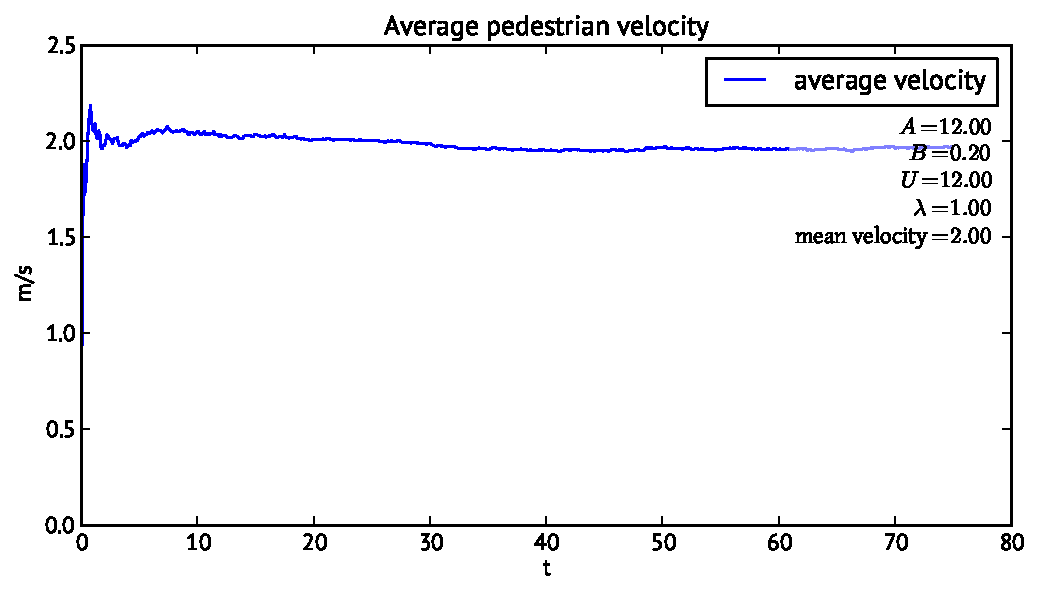
\includegraphics[scale=0.45]{Figures/normalcorridor-velocity.pdf}}
\subfloat[A graph of the mean velocity of the pedestrian in the corridor with a wide space]{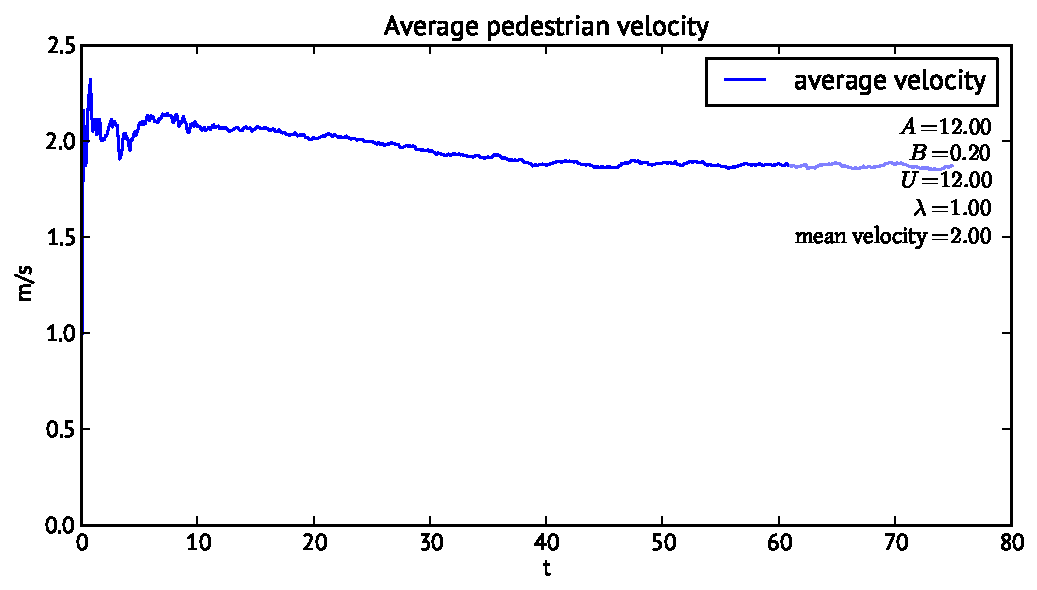
\includegraphics[scale=0.45]{Figures/Widekinkunidirec-velocity.pdf}}\\
\subfloat[A graph of the flow rate of the pedestrians in the normal corridor]{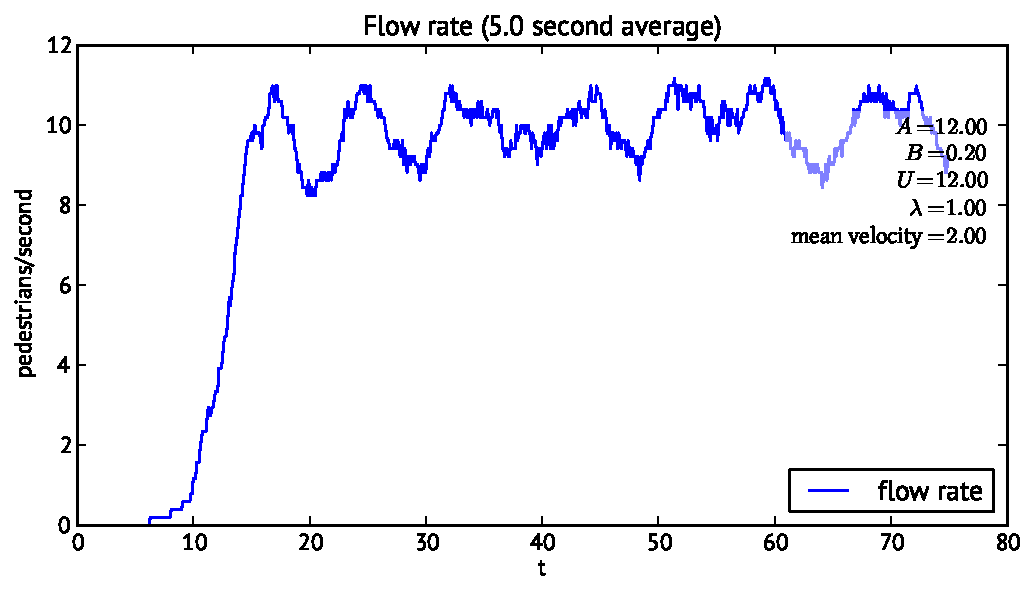
\includegraphics[scale=0.45]{Figures/normalcorridor-flowrate.pdf}}
\subfloat[A graph of the flowrate in the corridor with the wide space]{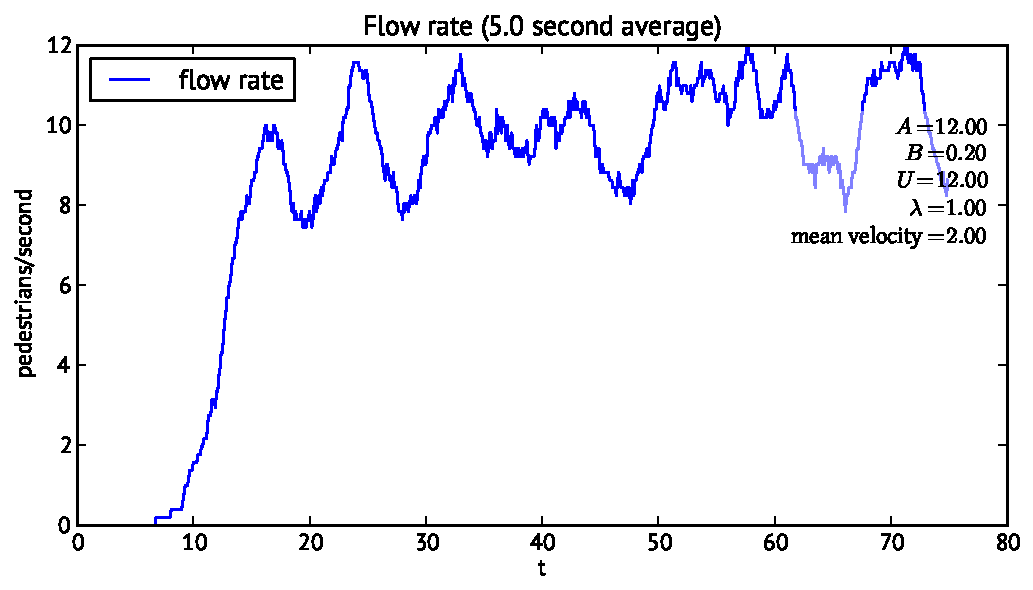
\includegraphics[scale=0.45]{Figures/Widekinkunidirec-flow.pdf}}
\caption{There is a lowering of the average velocity of the pedestrians due to the bottleneck. We see that there is no consistent lowering of the flowrate due to the bottleneck. What we see is that the flowrate is varying more over time.}
\label{fig:effect-of-widespace}
\end{figure}

\subsubsection{The faster-is-slower effect in the corridor with wide space}
The faster is slower effect in not observed in the extent that we would expect from 
the article. However the flow rate does not increase linearly with average velocity. 
 
\begin{figure}[h]
\centering
\subfloat[A graph of the flow rate as the average velocity is increased in the case of one directional pedestrian flow.]{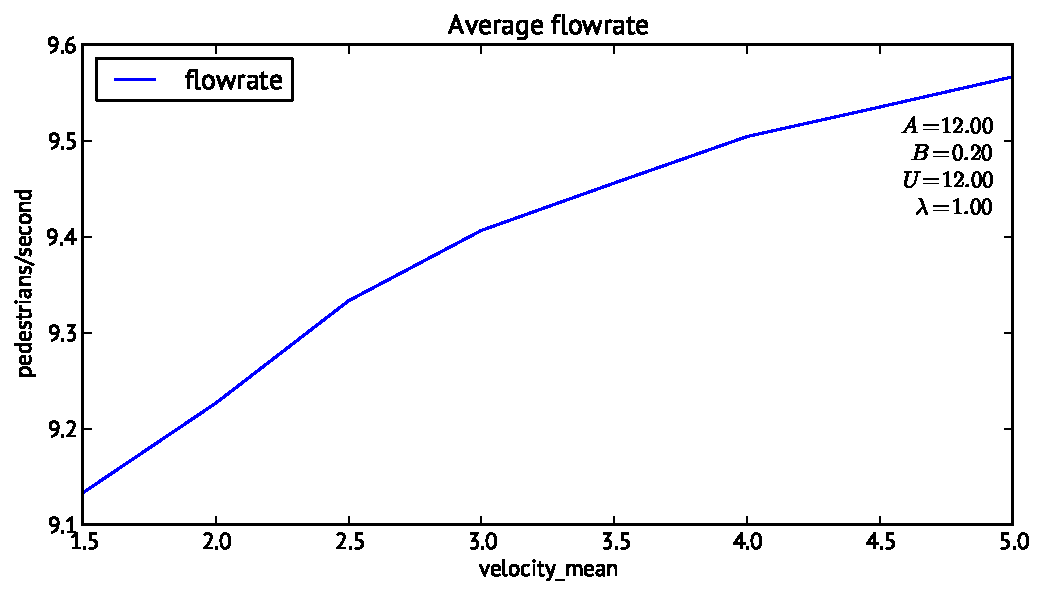
\includegraphics[scale=0.45]{Figures/Wide-kink-one-directional-flowrate-agg.pdf}}
\subfloat[A graph of the flow rate as the average velocity is increased in the case of bidirectional pedestrian flow.]{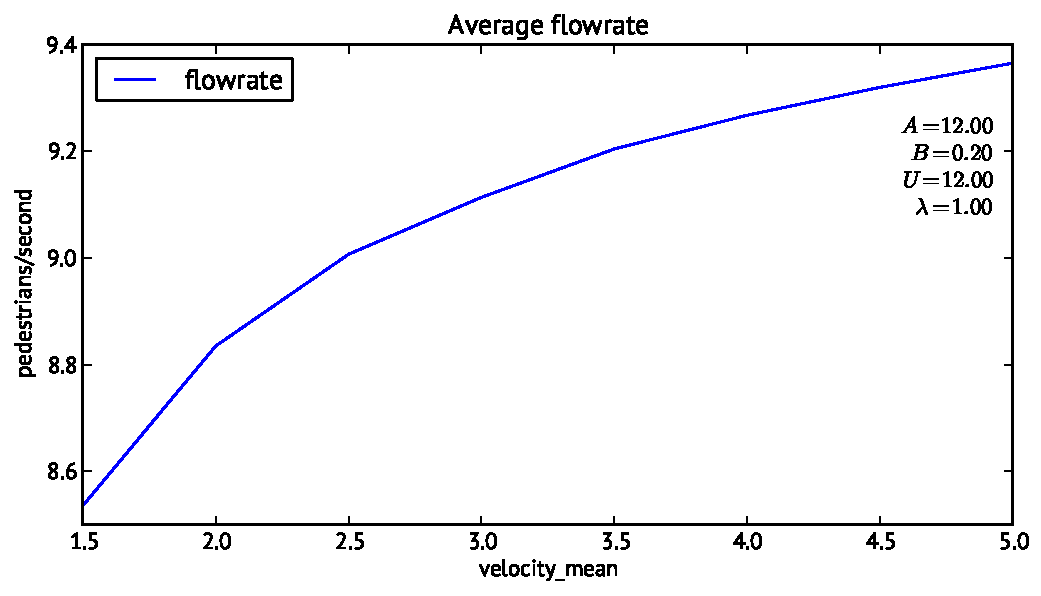
\includegraphics[scale=0.45]{Figures/Widekink-twodirectional-flowrate-agg.pdf}}
\caption{The two scenarios we want to compare to see the effect of the wide space.}
\label{fig:is-faster-slower-in-widekink}
\end{figure}

% TODO: Add parameters that are varied.
